\chapter{User Guide}

In this section it will be a briefly description of how to play the game.
The description will be described with text and some illustrations from the
game. 

\clearpage

\section{Game Elements}
	In this section, it will be a short description of the elements in the game.

	{\bf \#1: Power plant:} this building is the one that can serve the houses
	with power. A powerplant has a limited amount of power and can be upgarded
	in order to serve more buildings with power. Building a powerplant cost money.
	To serve buildings with power, the player is able to connect a power plant to
	buildings with power lines. \\
	{\bf \#2: Power lines: } this icon is the option when to choose when the player
	wants to build a powe line. \\
	{\bf \#3-\#7: Buildings: } this is the buildings that will appear randomly at the
	map at random intervals when the game starts. Each building require a different 
	amount of power and will also give the user a different amount of moeny. 
	The first building (\#1) will require least amount of power and the last building
	(\#7) will require the most amount power. \\
	{\bf \#8: Power line status:} in the game, a powerline can have three different kind
	of status. If a powerline is connected between two building without any connection
	to a powerplant, the line will be black and signalize that there is no power served
	to the buildings. If the buildings is not connected to a power plant, the buildings
	will dissapper and the health bar vil decrease. The Yellow line signalize that the
	houses is served with power and the user will be able to collect money. If the 
	power line is red, it signalize that the power line is damagesd/unstable. This is
	something that happends in the real world and the player needs to fix it so the
	houses can get power from the power plant. If it is not fixed, the houses will 
	dissappear and the healthbar will decrease. \\ 
	{\bf \#9: Coin: } this coin will appear next to a building when it is connected to
	a powerplant that can serve the building with power. This coin signalize that
	the building is buying power form the power plant. When this appear, the player
	is able to click on the building and collect the money in order to try to 
	reach the goal to get to the next level. 

	\begin{figure}[H]
		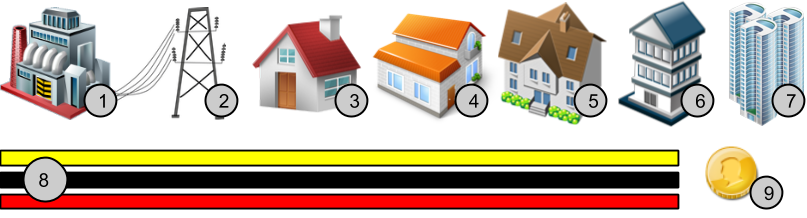
\includegraphics[width=\textwidth]{pictures/GameElements.png}
		\caption{Game elements}
	\end{figure}

\subsection*{Map Menu}
	When the game starts, there will be a menu in the buttom of the map. There 
	are a few elements in the menu the player needs to know:

	{\bf \#1 Money: } this is the amount of money the player have\\
	{\bf \#2 Goal: } is the amount of money the player needs to collect in 
	order to reach the next level.\\
	{\bf \#3 Healthbar: } is the health the player have. If it reached zero, it is game over. \\
	{\bf \#4 Build power plant: } is the element to choose if the player wants to build a power plant. \\
	{\bf \#5 Build power line: } is the element to choose if the player wants to build a powerline. \\
	{\bf \#6 Pause game: } the player can press this button to pause the game. \\

	\begin{figure}[H]
		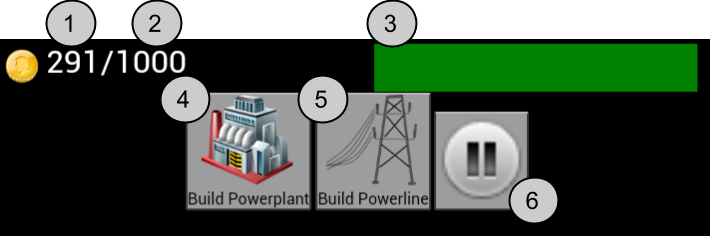
\includegraphics[width=\textwidth]{pictures/mapmenu.png}
		\caption{The map menu}
	\end{figure}

\subsection*{Start Game}
	The player is able to start the game by clicking on the "Power Supply" icon
	for the app at the phone. When the game starts, a flashscreen appears and the
	menu will show after 5 seconds. From the main menu, the player is able to 
	start a new game, see all highscores and read the instructions. 

	When the player starts a new game, a empty map will appear. When the game starts, 
	houses will start appearing a random positions at the map.

	The player need to build power plants, power lines and collect money in order
	to reach the next level.

\subsection*{Build Power Plant}

	When the game is started, a menu is showing in the bottom of the screen.
	From the main menu the player is able to choose to build a power plant.
	After selection "build power plant" the game is entering building mode and
	the player is able to choose the location to build the power plant. 

	In order to build a power plant, the player needs enough moeny and the
	location that is chosen have to be empty.

\subsection*{Build Power Line}

	When buildings appear at the map, the player is able to connect buildings and
	power plant with power lines. The player choose the "build power line" in the 
	menu and press on the buildings that the player want to connect. The first building
	will get a white circle around the building and after selecting the second one, there
	will appear a question if the player want to connect them or not.

\subsection*{Repair or remove damaged Power Line}

	If a powerline gets damaged, it will turn red. The player needs to press on the
	damaged powerline in order to fix it or remove it. 

\subsection*{Upgrade Power Plant}

	A power plant can only serve a fixed amount of power. If the player wants a power
	plant to serve more power, the player can a amount of money and upgrade the power plant. 
	When the player upgrades a power plant, it will be able to serve more houses with power.
	A power plant can only be upgraded up to level 5. A power plant can be upgraded by pressing
	on a power plant. 

\subsection*{Navigate around the map}
	
	The map in the game is quite big and the player needs to navigate around
	the map in order to get a overview of all the elements on the map. 
	In order to navigate, the player swipe the finger over the screen and the 
	map position will change. In order to get a full overview of the map, the player
	only needs to do a double-tap on the map. The map will then zoom out and the player
	can do a double-tap agian to go back to normal map view. 

\subsection*{Pause the game}

	If the player wants to pause the game, it is only to press the pause button in 
	the menu or just exit the game. 

\subsection*{Collect money}
	
	When buildings are connected to a power plant, the player will be able to collect
	money from the buildings. The player are able to collect the money by pressing on the
	building with a attached coin and the players amount of money will increase. If
	the amount of money is equal or greater than the goal, the player reaches the next level.

\subsection*{Building is not served with power}

	When a building appears on the map, a countdown starts. The player needs to connect
	the building to a power plant before the countdown is zero. If the countdown is zero, 
	the building will disappear and the health bar will decrease.  